%%%%%%%%%%%%%%%%%%%%%%%%%%%%%%%%%%%%%%%%%%%
%   Simple and elegant academic report    %
%   Copyright by Artur M. Brodzki, 2019   %
%%%%%%%%%%%%%%%%%%%%%%%%%%%%%%%%%%%%%%%%%%%

\documentclass{eiti-raport}

\usepackage[
	english,
	polish
]{babel}
\usepackage{polski}

%------------------------------------------

\begin{document}

\author{Artur M. Brodzki \\ Damian Chiliński \\ Krzysztof Sznejder}
\date{\today}
\subject{BCYB 19L}
\title{DNS Tunneling - dokumentacja koŃcowa}
\fancyhead[L]{Brodzki, Chiliński, Sznejder}
\fancyhead[R]{BCYB 19L}

\pagenumbering{arabic}
\maketitle

%------------------------------------------
% MAIN CONTENTS
%------------------------------------------

\section{Wstęp} \label{sec:intro}
Zgodnie z przyjętym przez nas tematem, celem projektu jest napisać moduł systemu IDS/IPS Snort, wykrywający steganograficzną transmisję danych metodą tunelowania DNS, oraz sprawdzić jego skuteczność. 

\section{Tunelowanie DNS} \label{sec:2}

\subsection{Zasada działania}
Tunelowanie DNS należy do metod steganograficznych i pozwala na prowadzenie niewidocznej dla administratorów transmisji danych, np. przesłanie na maszynę atakującego informacji wykradzionych z sieci korporacyjnej. Zasada działania opiera się na redundancji protokołu DNS. Typowy przebieg ataku z wykorzystaniem tunelowania DNS jest następujący:
\begin{enumerate}
	\item Atakujący rejestruje domenę, np. \texttt{bestmalware.win} i tworzy dla niej własny serwer autorytatywny. 
	\item Atakujący instaluje złośliwe oprogramowanie na systemach ofiary, które wykrada z nich wrażliwe dane, np. hasło bankowe. 
	\item Oprogramowanie atakującego koduje uzyskane informacje jako subdomenę, np: \\  \texttt{cXdlcnR5MTIzNDU2.bestmalware.win}, a następnie wysyła dla niej zapytanie DNS. Trafia ono na serwer atakującego, który może odebrać i zdekodować ukryte informacje. Dla uzyskania większego stopnia niewykrywalności, dane mogą być -- i zazwyczaj są -- szyfrowane przed wysłaniem. 
	\item Aby przeprowadzić transmisję w drugą stronę, wystarczy zakodować odpowiedź w rekordzie A/AAAA lub MX. Możliwe jest też wysyłanie większej ilości informacji w rekordach typu CNAME lub TXT. Takie rozwiązanie jest jednak raczej niestosowane z uwagi na łatwość wykrycia -- rekordy tego typu bardzo rzadko pojawiają się w ,,prawdziwym'' ruchu DNS. 
\end{enumerate}
Skuteczność tego rodzaju ataku bierze się z kluczowej roli, jaką odgrywa DNS w komunikacji internetowej. Jego zablokowanie może uniemożliwić działanie sieci, dlatego zapytania DNS bardzo rzadko są ograniczane przez administratorów, i to nawet w sieciach o restrykcyjnych wymogach bezpieczeństwa. 

\subsection{Metody wykrywania}
Aby skutecznie zwalczać ataki wykorzystujące tunelowanie DNS, konieczne jest wiarygodne odróżnienie złośliwych zapytań DNS od tych prawidłowych. Stosuje się w tym celu zbiór heurystyk, opartych m.in. o:
\begin{itemize}
	\item analizę długości i entropii zapytania;
	\item uczenie maszynowe: np. naiwny klasyfikator Bayesa oparty o n-gramy;
	\item analizę częstości: gwałtowny wzrost liczby wykonywanych zapytań DNS może sugerować, że znaczna ich część jest niepożądana;
	\item metody słownikowe. 
\end{itemize}
W naszym projekcie zamierzamy wykorzystać naiwny klasyfikator Bayesa oparty o analizę n-gramów, a w razie niedostatecznej skuteczności -- również inne metody, przede wszystkim analizę entropii i częstości zapytań. 

\section{Scenariusz projektowy}
W ramach projektu zamierzamy zrealizować następujący scenariusz: firma B-Cyb S.A. zarządza siecią korporacyjną, w której znajdują się serwery, hostujące publicznie dostępne usługi sieciowe. Sieć ta chroniona jest za pomocą systemu Snort oraz firewalla, zainstalowanego na firmowym routerze. Na firmowych serwerach znajduje się jednak złośliwe oprogramowanie, którego zadaniem jest przetransmitować na serwery atakującego wykradzione pliki \texttt{/etc/shadow} oraz \texttt{/etc/passwd}. Ponieważ firma B-Cyb obawia się ataku metodą tunelowania DNS, zakupiła od młodego zespołu specjalistów (Kant Security sp. z.o.o) dodatkowy moduł systemu Snort, mający wykrywać i blokować złośliwą transmisję. W ramach sieci firmowej została wydzielona podsieć, chroniona przy użyciu nowego modułu. 

\begin{figure} \centering
	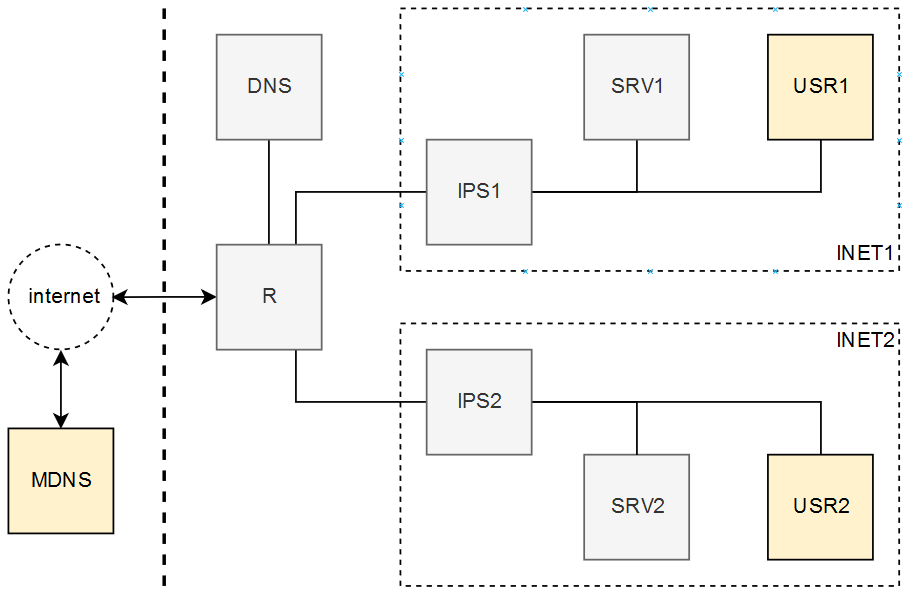
\includegraphics[width=0.9\linewidth]{img/BCYB-topologia.PNG}
	\label{fig:topologia}
	\caption{Schemat ideowy sieci, realizującej przyjęty scenariusz projektowy.}
\end{figure}

Całość infrastruktury została przedstawiona na rysunku 1. Składa się ona z następujących urządzeń: 
\begin{itemize}
	\item Router R: domyślna brama sieciowa dla sieci firmowej. Działa pod kontrolą systemu RouterOS i dostarcza zaporę sieciową (iptables), blokującą wszelki ruch wychodzący z firmowych serwerów, poza ruchem właściwym dla udostępnianych przez nie usług sieciowych. Przepuszczane są jednak  wychodzące z sieci zapytania DNS oraz HTTP, do określonych adresów -- umożliwia to chronionym maszynom pobieranie aktualizacji od zaufanych dostawców. 
	\item Firmowy serwer DNS: obsługujący lokalne zapytania. 
	\item Podsieć INET1, chroniona za pomocą dotychczasowej wersji systemu Snort:
	\begin{itemize}
		\item IPS1: host z uruchomionym systemem Snort, działającym w trybie \texttt{inline} i analizującym każdy pakiet wchodzący i wychodzący z głębiej położonych serwerów. 
		\item SRV1: serwer dostarczający niektóre z firmowych usług sieciowych. 
		\item USR1: komputer użytkowy, służący administratorowi firmy do zarządzania Snortem na maszynie IPS1, serwerem SRV1, oraz wykonywania pozostałych zadań administracyjnych. 
	\end{itemize}
	\item Podsieć INET2, chroniona za pomocą Snorta wyposażonego w nowo zakupiony moduł wykrywania tunelowania DNS:
	\begin{itemize}
		\item IPS2: host z uruchomionym systemem Snort, działającym w trybie \texttt{inline} i analizującym każdy pakiet wchodzący i wychodzący z głębiej położonych serwerów. 
		\item SRV2: serwer dostarczający niektóre z firmowych usług sieciowych. 
		\item USR2: komputer użytkowy, służący administratorowi firmy do zarządzania Snortem na maszynie IPS2, serwerem SRV2, oraz wykonywania pozostałych zadań administracyjnych. 
	\end{itemize}
\end{itemize}
Atakujący rejestruje własną domenę i tworzy dla niej serwer autorytatywny, oznaczony na rysunku 1 jako MDNS (ang. \textit{malicious DNS}). Stanowi on punkt odbiorczy ukrytej komunikacji. 

Cała opisana powyżej infrastruktura zostanie przez nas zwirtualizowana za pomocą programów VirtualBox oraz Vagrant i możliwa będzie do uruchomienia na jednej fizycznej maszynie\footnote{Posiadającej co najmniej 16 GB pamięci RAM.}. Maszyny wirtualne oznaczone na rysunku 1 kolorem szarym działają w tle i dostęp do nich jest możliwy tylko przez SSH. Natomiast maszyny oznaczone kolorem żółtym uruchamiane są w trybie graficznym i służą do zaprezentowania następującego scenariusza:
\begin{itemize}
	\item W sieci INET1 możliwe jest przeglądanie HTTP z komputera USR1 -- ruch DNS i HTTP/HTTPS nie jest blokowany. Jednocześnie niemożliwe jest inicjowanie ruchu wychodzącego z serwera SRV1 -- jest on blokowany przez zaporę sieciową. 
	\item Sieć INET2 chroniona jest przez dodatkowy moduł systemu Snort. Przeglądanie HTTP z komputera USR2 nadal jest możliwe -- nieszkodliwe zapytania DNS są poprawnie rozpoznawane i nie podlegają blokowaniu. Podobnie jak w sieci INET1, niemożliwe jest inicjowanie ruchu z serwera SRV2. 
	\item Atakujący działa na maszynie MDNS. Może on obejrzeć w przeglądarce publicznie dostępną zawartość serwerów SRV1 i SRV2. Podejmuje on również próbę przechwycenia wrażliwych danych z maszyny SRV1 oraz SRV2. O ile udaje mu się to w przypadku SRV1, to w przypadku SRV2 próba transmisji zostaje wykryta i zablokowana przez przygotowany moduł systemu Snort. 
\end{itemize}
Opisana wyżej sekwencja działań stanowi ramowy plan prezentacji, którą przedstawimy na zakończenie projektu. 

\section{Podsumowanie} \label{sec:summary}
Tak przygotowany scenariusz projektowy pozwoli nam na przetestowanie możliwości wykrywania tunelowania DNS z wykorzystaniem uczenia maszynowego oraz zaprezentowanie działania systemów typu IDS/IPS w praktyce. 

\end{document}
